%!tex root=./thesis.tex
\chapter{Faraday Complexity}
\label{cha:faraday-faraday}

\section{Faraday Complexity}
\label{sec:faraday-faraday-complexity}

This chapter is based on my to-be-submitted paper \emph{Interpretable Faraday Complexity Classification}, by M. J. Alger, C. S. Ong, J. D. Livingston, J. L. Nabaglo, N. M. McClure-Griffiths, and O. I. Wong.

  Quickly determining the Faraday complexity of a spectropolarimetric observation is important for processing large, polarised radio surveys. Finding simple sources lets us build rotation measure grids, and finding complex sources lets us follow these sources up with slower analysis techniques or further observations. We introduce a simple, interpretable machine learning method for estimating Faraday complexity. We train this method on simulated polarised radio observations and analyse its behaviour, and demonstrate our method on both simulated and real data. With 95 per cent accuracy on simulated data, our method performs comparably to state-of-the-art convolutional neural networks while being simpler and easier to interpret. The method behaves sensibly on real data and gives plausible Faraday complexity classifications.

\section{Introduction}
\label{sec:faraday-intro}

  As polarised radiation from distant galaxies makes its way to us, magnetised plasma along the way can cause the polarisation angle to change due to the Faraday effect. The amount of rotation depends on the squared wavelength of the radiation, and the rotation per squared wavelength is called the Faraday depth. The Faraday depth is related to the electron density and the magnetic field strength:
  \begin{equation}
      \phi = 0.81 \int_{\mathrm{there}}^{\mathrm{here}} n_e(\vec r) \vec B(\vec r) \cdot \mathrm{d}\vec{r}\ \mathrm{rad}\ \mathrm{m}^{-2}.
  \end{equation}
  Here $\phi$ is the Faraday depth, $n_e$ is the electron density in $\mathrm{cm}^{-3}$, $\vec B$ is the magnetic field in $\upmu$G, and $\mathrm{d}\vec r$ is the infinitesimal path length in pc \citep{brentjens_faraday_2005}. Multiple Faraday depths may exist along one line-of-sight, and if a polarised source is observed at multiple wavelengths then these multiple depths can be disentangled. This can provide insight into the polarised structure of the source.

  Faraday rotation measure synthesis (RM synthesis) is a technique for decomposing a spectropolarimetric observation into flux at its Faraday depths $\phi$, the resulting distribution of depths being called a `Faraday dispersion function' (FDF) or a `Faraday spectrum'. It was introduced by \citet{brentjens_faraday_2005} as a way to rapidly and reliably analyse the polarisation structure of complex and high-Faraday depth polarised observations. The relationship between the observed complex polarised surface brightness $P(\lambda^2)$ and the underlying FDF $F(\phi)$ is similar to a Fourier transform:

  \begin{equation}
      \label{eq:faraday-f-to-p}
      P(\lambda^2) = \int_{-\infty}^{\infty} F(\phi) e^{2i\phi\lambda^2}\ \mathrm{d}\phi.
  \end{equation}

  $\lambda^2$ is the squared radiation wavelength. A `Faraday simple' observation is one for which there is only one Faraday depth. Equivalently, the polarisation angle $\chi(\lambda^2)$ changes linearly with $\lambda^2$ with the Faraday depth as the gradient, i.e.:
  \begin{equation}
    \label{eq:faraday-chi}
    \chi(\lambda^2) = \chi_0 + \phi \lambda^2.    
  \end{equation}
  In this case, the Faraday depth is also called the `rotation measure' (RM).

  All Faraday simple observations can be modelled as a polarised source with a magnetised thermal plasma \citep[a `Faraday screen';][]{brentjens_faraday_2005,anderson_broadband_2015} between the observer and the source. A `Faraday complex' observation is one which is not Faraday simple, and may differ from a Faraday simple source due to plasma emission or composition of multiple screens \citep{brentjens_faraday_2005}. The complexity of a source tells us important details about the polarised structure along the line-of-sight, such as whether the intervening medium emits polarised radiation, or whether there is turbulent magnetic fields or different electron densities in the neighbourhood. The complexity of nearby sources taken together tells us about the magneto-ionic structure of the galactic and intergalactic medium between the sources and us as observers.

  Identifying when an observation is Faraday complex is an important problem in polarised surveys, and with surveys now being conducted larger than ever before, methods that can quickly characterise Faraday complexity en masse are increasingly useful. Being able to identify which sources are simple lets us produce a reliable rotation measure grid from background sources, and being able to identify which sources might be complex allows us to find sources to follow-up with slower polarisation analysis methods that may require manual oversight. We introduce a simple, interpretable method for estimating Faraday complexity, building interpretable features for observed polarised sources by comparing them to idealised polarised sources. These features are easy to understand and can be estimated from real FDFs. We demonstrate the effectiveness of our method on both simulated and real data. Using simulated data, we compare our method to the state-of-the-art CNN Faraday complexity estimation methods.

\section{Faraday dispersion functions}

  \begin{figure}
    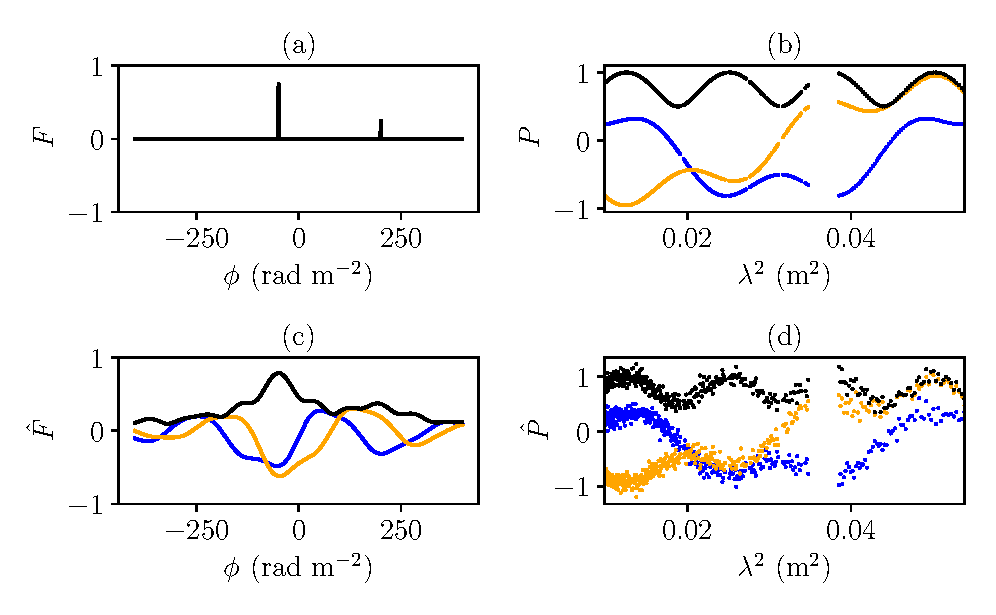
\includegraphics[width=\linewidth]{faraday-images/spectra.pdf}
    \caption{A complex FDF and its corresponding polarised spectra: (a) groundtruth FDF $F$, (b) noise-free polarised spectrum $P$, (c) noisy observed FDF $\hat F$, (d) noisy polarised spectrum $\hat P$. Blue and orange mark real and imaginary components respectively.}
  \end{figure}

  \begin{figure}
    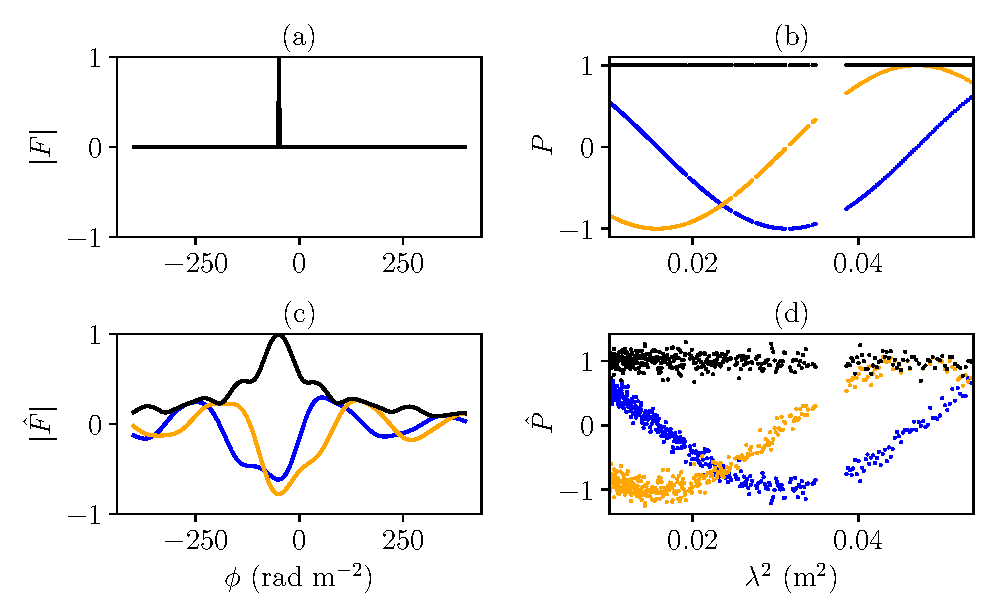
\includegraphics[width=\linewidth]{faraday-images/spectra_simple.pdf}
    \caption{A simple FDF and its corresponding polarised spectra: (a) groundtruth FDF $F$, (b) noise-free polarised spectrum $P$, (c) noisy observed FDF $\hat F$, (d) noisy polarised spectrum $\hat P$. Blue and orange mark real and imaginary components respectively.}
  \end{figure}

  \begin{figure}
    \includegraphics[width=\linewidth]{faraday-images/rmsf.pdf}
    \caption{A RMSF $R(\phi)$. Blue and orange mark real and imaginary components respectively.}
    \label{fig:faraday-rmsf}
  \end{figure}

  For the purposes of this paper, an FDF is a function $F$ from Faraday depth $\phi$ to complex polarisation. The FDF is implicitly defined and related to the polarised spectrum $P$ by \autoref{eq:f-to-p}. It is the distribution of Faraday depths in the observed source. We assume that $F$ has no noise and no observational limitations, and so $P$ also has no noise or limitations. We instead define $\hat F$ and $\hat P$ as the noisy, observed FDF and polarisation respectively. $\hat P$ is observed directly, and $\hat F$ is defined in terms of $\hat P$ by RM synthesis:
  \begin{equation}
      \label{eq:faraday-rm-synthesis}
      \hat F(\phi) = K^{-1} \int_{0}^{\infty} W(\lambda^2) \hat P(\lambda^2) e^{-2i\phi\lambda^2}\ \mathrm{d}\lambda^2.
  \end{equation}
  $W(\lambda^2)$ is a weighting function, which we assume to be 1 if polarisation was observed at $\lambda^2$ and 0 for all other values. This is called `uniform weighting' and is the most common weighting function for RM synthesis, but other weighting functions are possible in analogy with radio synthesis imaging. $K$ is a normalisation constant:
  \begin{equation}
    \label{eq:faraday-k}
    K = \int_{0}^\infty W(\lambda^2)\ \mathrm{d}\lambda^2.
  \end{equation}
  \citet{brentjens_faraday_2005} show that when there is no noise, the observed FDF $\hat F$ is related to the groundtruth $F$ by convolution with a function $R$ called the `rotation measure spread function' or RMSF:
  \begin{equation}
    \label{eq:faraday-hat-f-r-ast-f}
    \hat F(\phi) \overset{\text{no noise}}{=} (R \ast F)(\phi)
  \end{equation}
  $R$ is defined as the normalised Fourier transform of $W$:
  \begin{equation}
    \label{eq:faraday-rmsf}
    R(\phi) = K^{-1} \int_{0}^{\infty} W(\lambda^2) e^{-2i\phi\lambda^2}\ \mathrm{d}{\lambda^2}.
  \end{equation}
  If the noise in $\hat P$ is wavelength-independent Gaussian, then $\hat F$ can be represented as a Gaussian process with kernel $R$ and mean $R \ast F$. In other words,
  \begin{equation}
    \label{eq:faraday-hat-f-distribution}
    p(\hat F) = \mathcal N_c(\hat F \mid R \ast F, \Sigma(\phi, \varphi))
  \end{equation}
  where the covariance $\Sigma$ is
  \begin{equation}
    \Sigma(\phi, \varphi) = \int_{-\infty}^\infty R(\vartheta - \phi) R(\vartheta - \varphi)\ \mathrm{d}\vartheta.
  \end{equation}
  Note that there are two reasons that the observed FDF does not match the groundtruth FDF. The first is the noise in $\hat P$. The second arises from the incomplete sampling of $\hat P$ as represented by $W$. In summary, $F$ is the groundtruth FDF, $P$ is the noise-free polarisation spectrum, $\hat P$ is the noisy/observed polarisation spectrum, $\hat F$ is the noisy/observed FDF, $W$ is a weighting function and $R$ is the RMSF. Observations $\hat F$ can be simulated by either performing RM synthesis on simulated polarisation spectra or by drawing from \autoref{eq:hat-f-distribution}.

  % Assuming uncorrelated Gaussian noise in the polarised signal, $\hat P$ is drawn from a degenerate Gaussian process:
  % \begin{equation}
  %   \label{eq:faraday-hat-p}
  %   \hat P(\lambda^2) \sim W(\lambda^2) \left[P(\lambda^2) + \epsilon(\lambda^2)\right].
  % \end{equation}
  % $\epsilon : \mathbb R \to \mathbb C$ is a zero-mean, ergodic, and uncorrelated (white) Gaussian process, and $W(\lambda^2)$ is 1 if we observed at $\lambda^2$ and 0 for all other values. Note that we assume uniform weighting for RM synthesis throughout this paper. Also, in general, the Gaussian noise in $\hat P$ may not be uncorrelated and may not be ergodic.

  \subsection{Assumptions on polarised sources}
  \label{sec:faraday-assumptions}

    For the simulation and calculations in this paper, we make a number of simplifications to limit the scope of Faraday dispersion functions considered. These simplifications are not unphysical, though real sources may have additional complications which we discuss later. We assume that all polarised sources are composed of either one or two Faraday screens. This accounts for most actual sources \citep{anderson_broadband_2015} and extension to three screens would cover most of the remainder---\citet{osullivan_broad-band_2017} found that 91 per cent of their sources were best explained by two or less screens, while the remainder were best explained by three screens. This means that every groundtruth FDF is of the form
    \begin{equation}
        \label{eq:faraday-true-fdf}
        F(\phi) = A_0 \delta(\phi - \phi_0) + A_1 \delta(\phi - \phi_1).
    \end{equation}
    With this model, a Faraday simple source is one which has $A_0 = 0$, $A_1 = 1$, or $\phi_0 = \phi_1$. Applying \autoref{eq:f-to-p}, every noise-free polarised spectrum is of the form
    \begin{equation}
        \label{eq:faraday-true-pol}
        P(\lambda^2) = A_0 e^{2i\phi_0\lambda^2} + A_1 e^{2i\phi_1\lambda^2}.
    \end{equation}
    We assume that polarised observations $\hat P$ have complex Gaussian noise $\epsilon$:
    \begin{align}
        \label{eq:faraday-pol-noise}
        \epsilon(\lambda^2) \sim \mathcal N_c(0, \sigma^2),
    \end{align}
    where $\sigma^2$ is constant. The constant variance of the noise is a simplifying assumption which may not hold for real data, and exploring this is a topic for future work.

    We do not consider external or internal Faraday dispersion in this work. External Faraday dispersion would broaden the delta functions of \autoref{eq:true-fdf} into peaks, and internal Faraday dispersion would broaden them into top-hat functions. All sources have at least a small amount of dispersion as the Faraday depth is a bulk property of the intervening medium and is subject to noise, but the assumption we make is that this dispersion is sufficiently small that the groundtruth FDFs are well-modelled with delta functions. Faraday thick sources would also invalidate our assumptions, and we assume that there are none in our data as Faraday thickness is hard to observe anyway \citeneeded.

  \subsection{Simulating observed FDFs}
  \label{sec:faraday-simulated-fdfs}

    To simulate observed FDFs we follow the method of \citet{brown_classifying_2018}. $F$ is approximated on the domain $[\phi_{\min}, \phi_{\max}]$ by a vector $\vec F \in \mathbb R^d$:
    \begin{equation}
      \label{eq:faraday-vec-f}
      \vec F_j = \sum_{k = 0}^1 A_k \delta(\phi_{\min} + j \delta \phi - \phi_k)
    \end{equation}
    where $\delta\phi = (\phi_{\max} - \phi_{\min}) / d$ and $d$ is the number of Faraday depth samples in the FDF.
    $\vec F$ is sampled by uniformly sampling its parameters:
    \begin{align}
      \label{eq:faraday-model-distributions}
      % p(\phi_0, \phi_1, A_0, A_1) = \frac{1}{(\phi_{\max} - \phi_{\min})^2} \begin{cases}
      %   1 & \phi_{0,1} \in [\phi_{\min} \phi_{\max}],\\
      %     & A_{0, 1} \in [0, 1];\\
      %   0 & \mathrm{otherwise}.
      % \end{cases}
      % p(\phi_k) &= \frac{1}{\phi_{\max} - \phi_{\min}} \begin{cases}
      %   1 & \phi_k \in [\phi_{\min} \phi_{\max}],\\
      %   0 & \mathrm{otherwise};
      % \end{cases}\\
      % p(A_k) &= \begin{cases}
      %   1 & \phi_k \in [0, 1],\\
      %   0 & \mathrm{otherwise};
      % \end{cases}
      \phi_k &\in [\phi_{\min}, \phi_{\min} + \delta\phi, \dots, \phi_{\max}]\\
      A_k &\sim \mathcal U(0, 1).
    \end{align}
    We assume that the total polarisation is 1: real observations can be scaled to this by dividing by their total polarisation. We then generate a vector polarisation spectrum $\vec P \in \mathbb R^m$ from $\vec F$ using a discretised \autoref{eq:f-to-p}:
    \begin{equation}
      \label{eq:faraday-discrete-f-to-p}
      \vec P_\ell = \sum_{j = 0}^{j} F_j e^{2i(\phi_{\min} + j\delta_\phi)\lambda^2_\ell}\ \mathrm{d}\phi.
    \end{equation}
    $\lambda^2_\ell$ is the discretised value of $\lambda^2$ at the $\ell$th index of $\vec P$. This requires a set of $\lambda^2$ values, which depends on the dataset being simulated. In this paper we use two different sets of $\lambda^2$ values, which we detail later in \autoref{sec:experiment-classification}. These values can be treated as the channel wavelengths at which the polarisation spectrum was observed. We then add Gaussian noise with variance $\sigma^2$ to each element of $\vec P$ to obtain a discretised noisy observation $\hat{\vec{P}}$. Finally, we perform RM synthesis using the Canadian Initiative for Radio Astronomy Data Analysis \texttt{RM} package\footnote{\url{https://github.com/CIRADA-Tools/RM}}, which is a \texttt{Python} module that implements a discrete version of RM synthesis:
    \begin{equation}
      \label{eq:faraday-discrete-rm-synthesis}
      \hat{\vec{F}}_j = m^{-1} \sum_{\ell = 1}^m \vec{\hat P}_\ell e^{-2i(\phi_{\min} + j\delta_\phi)\lambda^2_\ell}.
    \end{equation}

\section{Faraday complexity}

    Faraday complexity is an observational property of a source: if multiple Faraday depths are observed within the same apparent source (e.g. due to multiple lines-of-sight being combined within a beam), then the source is complex, and otherwise it is simple. Faraday thickness is also a source of Faraday complexity: when the intervening medium between a polarised source and the observer also emits polarised light, the FDF can not be characterised by a simple Faraday screen. As per \autoref{sec:assumptions} we defer Faraday thick sources to future work. A source composed of multiple Faraday screens may be consistent with many other models \citep{sun15comparison}, including simple sources, so there is some overlap between simple and complex sources.

    There are multiple ways to estimate Faraday complexity, including detecting non-linearity in $\chi(\lambda^2)$ \citep{goldstein84faraday}, change in fractional polarisation as a function of frequency \citep{farnes14broadband}, non-sinusoidal variation in fractional polarisation in Stokes $Q$ and $U$ \citep{osullivan12agn}, counting components in the FDF \citep{law11faraday}, minimising the Bayesian information criterion (BIC) over a range of simple and complex models \citep[called `QU fitting'][]{osullivan_broad-band_2017}, the method of Faraday moments \citep{anderson_broadband_2015,Brown11report}, and deep convolutional neural network classifiers \citep[CNNs;][]{brown_classifying_2018}. See \citep{sun15comparison} for some discussion of these methods.

    \subsection{Methods for estimating complexity}
    \label{sec:faraday-existing-methods}

        Faraday moments \citep{Brown11report,anderson_broadband_2015} and CNNs \citep{brown_classifying_2018} are the two methods for estimating Faraday moments that we will consider here.

        \subsubsection{Faraday moments}
        \label{sec:faraday-faraday-moments}
            The method of Faraday moments requires the FDF to be deconvolved using \texttt{RM-CLEAN} \citep{heald09faraday}, a deconvolution program in analogy to \texttt{CLEAN} used in radio synthesis imagery. The estimated deconvolved FDF is a sum of delta functions called `clean components'. The second moment is computed over these components and thresholded to determine if a source is Faraday complex. The second moment $\varsigma_{\mathrm{mom}}$ is defined as
            \begin{equation}
                \varsigma_{\mathrm{mom}}^2 = K_C^{-1} \sum_{i = 1}^N (\phi_i - \langle \phi \rangle)^2 |C_i|
            \end{equation}
            where $N$ is the number of clean components, $C_i$ is the complex intensity of the $i$th clean component, $K_C$ is the normalisation:
            \begin{equation}
                K_C = \sum_{i = 1}^N |C_i|,
            \end{equation}
            and $\langle \phi \rangle$ is the mean depth of the clean components:
            \begin{equation}
                \langle \phi \rangle = K_C^{-1} \sum_{i = 1}^N \phi_i |C_i|.
            \end{equation}
            A non-zero Faraday moment means that the source is Faraday complex. However, a zero Faraday moment may still be consistent with a complex source, so a zero Faraday moment does not mean that the source must be Faraday simple.

            Drawbacks of this method include the need to determine a threshold and the care required to produce the clean components. In particular, deconvolution is a challenging process and works poorly on noisy data. Significant oversight is required to clean large quantities of sources, which limits its usage in large surveys.

            For our model spectra (\autoref{eq:true-fdf}) we can treat each delta function as a clean component and hence write down the Faraday moment for a FDF in the ideal, fully-observed scenario (i.e. no noise and an infinitely thin RMSF):
            \begin{equation}
                \label{eq:faraday-model-moment}
                \varsigma_{\mathrm{mom}}^2 = \frac{A_0A_1}{(A_0 + A_1)^2} (\phi_0 - \phi_1)^2.
            \end{equation}
            This has units of rad~m$^{-2}$.

        \subsubsection{Convolutional neural networks}
        \label{sec:faraday-cnns}

          Convolutional neural networks (CNNs) are a variant of neural networks that are designed for prediction on data with local correlations, such as spectra and images. CNNs have recently gained popularity in astroinformatics thanks to their success on large image datasets \citep[e.g.][]{lukic18compact} and spectral datasets \citep[e.g.][]{muthukrishna19dash}. \citet{brown_classifying_2018} employ an inception network \citep{szegedy15deeper} CNNs to estimate Faraday complexity of simulated FDFs. The CNN outputs a probability that a source is complex or simple. Drawbacks of this method include slow training time and difficulty in understanding how the CNN decides on its output.

    \subsection{Features for classifying complexity}
    \label{sec:faraday-scores-method}

      The Faraday complexity classification problem is as follows: Given a FDF $\hat F$, is it Faraday complex or Faraday simple?

      We developed a classifier $\varsigma : \mathbb R^k \to \mathbb R$ which takes as input a $k$-dimensional vector representing an FDF, and outputs the probability that the FDF is complex. As input we needed a representation of the FDF, and for this we used five features derived from the distance between the FDF and the manifold of simple FDFs. This is a sensible characterisation because when the distance is zero the FDF lies on the simple manifold and hence the FDF must be simple, and the distance increases as the FDF becomes more complex. Under some distance measure $D_f$, the distance to the simple manifold is
      \begin{equation}
          \label{eq:faraday-complexity-model}
          \varsigma_f(\hat F) = \min_{\phi_w \in \mathbb{R}} D_f\infdivx{\hat F(\phi)}{\hat F_{\mathrm{simple}}(\phi; \phi_s)}
      \end{equation}
      where $\hat F_{\mathrm{simple}}$ is a simulated simple FDF with no noise and a Faraday depth of $\phi_s$:
      \begin{align}
          \label{eq:faraday-f-simple}
          F_{\mathrm{simple}}(\phi; \phi_s) &= \delta(\phi - \phi_s)\\
          \hat F_{\mathrm{simple}}(\phi; \phi_s) &= R(\phi - \phi_s).
      \end{align}
      $\hat F_{\mathrm{simple}}$ parametrises the simple manifold. This distance has nice properties, as it is:
      \begin{itemize}
          \item phase-invariant,
          \item translationally invariant in Faraday depth,
          \item zero for Faraday simple sources (i.e. when $A_0 = 0$, $A_1 = 0$, or $\phi_0 = \phi_1$) when there is no noise,
          \item symmetric in components (i.e. swapping $A_0 \leftrightarrow A_1$ and $\phi_0 \leftrightarrow \phi_1$ should not change the distance),
          \item increasing as $A_0$ and $A_1$ become closer to each other, and
          \item increasing as screen separation $|\phi_0 - \phi_1|$ increases over a large range.
      \end{itemize}

      While we could choose any functional distance measure, we mainly used the 2-Wasserstein ($W_2$) distance. Under this choice of distance, the minimiser $\phi_s$ in \autoref{eq:complexity-model} can be interpreted as the Faraday depth that the FDF $\hat F$ would be observed to have if its complexity was unresolved (i.e. the weighted mean of its components). In the case where there is no RMSF, \autoref{eq:complexity-model} reduces to the Faraday moment already in common use:
      \begin{align}
          D_{W_2}(F) &= \min_{\phi_w \in \mathbb{R}} D_{W_2}\infdivx{F(\phi)}{F_{\mathrm{simple}}(\phi; \phi_w)}\\
              &= \left(\frac{A_0A_1}{(A_0 + A_1)^2} (\phi_0 - \phi_1)^2\right)^{1/2}.
      \end{align}
      See \autoref{sec:w2-to-faraday-moments} for the corresponding calculation. In this sense, the $W_2$ distance can be thought of as a generalised Faraday moment. Interestingly, this also provides an interpretation of Faraday moments as a distance from the simple manifold in the case where there is no RMSF.

      The $W_2$ distance, usually defined on probability distributions, can be extended to one-dimensional complex functions $A$ and $B$ by normalising them:
      \begin{align}
        \label{eq:faraday-w2}
        D_{W_2}\infdivx{A}{B}^2 &= \inf_{\gamma \in \Gamma(A, B)} \iint_{\phi_{\min}}^{\phi_{\max}} |x - y|^2\ \mathrm{d}\gamma(x, y) \\
        \label{eq:faraday-normalised}
        \tilde A(\phi) &= \frac{|A(\phi)|}{\int_{\phi_{\min}}^{\phi_{\max}} |A(\theta)|\ \mathrm{d}\theta}\\
        \tilde B(\phi) &= \frac{|B(\phi)|}{\int_{\phi_{\min}}^{\phi_{\max}} |B(\theta)|\ \mathrm{d}\theta}
      \end{align}
      where $\Gamma(A, B)$ is the set of couplings of $A$ and $B$, i.e. the set of joint probability distributions that marginalise to $A$ and $B$. This can be interpreted as the minimum cost to `move' one probability distribution to the other, where the cost of moving one unit of probability mass is the squared distance it is moved. We calculated the $W_2$ distance using \texttt{Python Optimal Transport} \citep{flamary17pot}, which uses a method summarised in \autoref{sec:pot}.

      We also made use of the Euclidean distance to the simple manifold:
      \begin{equation}
        \label{eq:faraday-euclidean}
        D_E\infdivx{A}{B}^2 = \int_{\phi_{\min}}^{\phi_{\max}} |x - y|^2\ \mathrm{d}\phi.\\
      \end{equation}
      It is the least-squares loss of fitting a simple FDF to the observed FDF. In the case where there is no RMSF, the Euclidean distance becomes
      \begin{align}
          D_{E}(F) &= \min_{\phi_e \in \mathbb{R}} D_E\infdivx{F(\phi)}{F_{\mathrm{simple}}(\phi; \phi_e)}\\
              &= \sqrt{2} \frac{\min(A_0, A_1)}{A_0 + A_1}.
      \end{align}
      See \autoref{sec:euclidean-calculation} for the corresponding calculation. Note that there is no reference to the Faraday depths of the FDF components in the Euclidean distance---dependence is only on the amplitudes of the components. We found the Euclidean distance using \texttt{scipy.spatial.distance.euclidean} \citep{scipy2020}.

      To generate the five features representing an FDF $\hat F$, we first found the closest simple FDF $\hat F_{\mathrm{simple}}(\phi; \phi_w)$ to $\hat F$ using $W_2$ distance:
      \begin{equation}
        \phi_w = \underset{\phi_w}{\mathrm{argmin}}\ D_{W_2}\infdivx{\hat F(\phi)}{\hat F_{\mathrm{simple}}(\phi; \phi_w)}.
      \end{equation}
      $\phi_w$ is interpretable as the value of Faraday depth that one would observe if the Faraday-space resolution is too low to observe Faraday depth, i.e., if a multi-component FDF is unresolved. We also found the Faraday depth of the largest peak:
      \begin{equation}
        \phi_a = \underset{\phi_a}{\mathrm{argmax}}\ |\hat F(\phi_a)|,
      \end{equation}
      as well as the closest simple FDF using Euclidean distance:
      \begin{equation}
        \phi_e = \underset{\phi_e}{\mathrm{argmin}}\ D_E\infdivx{\hat F(\phi)}{\hat F_{\mathrm{simple}}(\phi; \phi_e)}.
      \end{equation}

      \begin{figure}
        \centering
        \includegraphics[width=\linewidth]{faraday-images/features_simparams.pdf}
        \caption{\label{fig:faraday-features-simparams} Features as a function of properties of simulated FDFs. $\Delta \phi$ is the component separation and $\min(A_0, A_1)$ is the minimum component amplitude.}
      \end{figure}

      From these Faraday depths we generate five features:
      \begin{itemize}
        \item $\log |\phi_w - \phi_a|$,
        \item $\log \hat F(\phi_w)$,
        \item $\log \hat F(\phi_a; \phi_w)$,
        \item $\log D_{W_2}\infdivx{\hat F(\phi)}{\hat F_{\mathrm{simple}}(\phi; \phi_w)}$,
        \item $\log D_{E}\infdivx{\hat F(\phi)}{\hat F_{\mathrm{simple}}(\phi; \phi_e)}$.
      \end{itemize}
      The relationship between these features and the Faraday screens in our simulation is shown in \autoref{fig:features-simparams}.

      We can then train any off-the-shelf classifier on these features to obtain a Faraday complexity classifier. We describe our classifiers in \autoref{sec:classifiers}.

% \section{Experiment: No noise}

%   \begin{figure}
%     \centering
%     % \includegraphics[width=\linewidth]{faraday-images/complexities_abcd_3d.pdf}
%     \includegraphics[width=\linewidth]{faraday-images/complexities_a_3d.pdf}
%     \includegraphics[width=\linewidth]{faraday-images/complexities_b_3d.pdf}
%     \includegraphics[width=\linewidth]{faraday-images/complexities_c_3d.pdf}
%     \includegraphics[width=\linewidth]{faraday-images/complexities_d_3d.pdf}
%     \includegraphics[width=\linewidth]{faraday-images/complexities_e_3d.pdf}
%     \caption{Faraday complexity scores derived from different divergences. All plots are shown with arbitrary linear scales.}
%     \label{fig:faraday-no-noise-complexities}
%   \end{figure}
  
%   We begin by examining the behaviour of different Faraday complexity scores in the case where there is no noise, i.e. $\epsilon = 0$. In this setting the only difference between the groundtruth FDF and the observed FDF is the RMSF, so \autoref{eq:hat-f-r-ast-f} holds exactly. We generated 2~000 FDFs $\hat{\vec{F}}$ with different amplitudes and Faraday depths. For each divergence measure (Euclidean, KL, IS, and W$_2$) we calculated the corresponding Faraday complexity score for each FDF ($\varsigma_{\mathrm{Euc}}, \varsigma_{\mathrm{KL}}, \varsigma_{\mathrm{IS}},$ and $\varsigma_{\mathcal E}$ respectively) following \autoref{eq:complexity-observed}. We also calculated the Faraday moment ($\varsigma_{\mathrm{mom}}$, \autoref{eq:model-moment}) of the true FDFs $\vec F$. The Faraday complexity scores are plotted in \autoref{fig:no-noise-complexities}. For this experiment, we use the frequency coverage of Livingston (in prep), the RMSF of which is plotted in \autoref{fig:rmsf}.

%   Visually, W$_2$ best approximates the Faraday moment. This can be confirmed by computing the Spearman $\rho$ coefficient \citeneeded{} of the Faraday complexity score compared to the Faraday moment. W$_2$ has the highest Spearman $\rho$ of $\rho = 0.887$, followed by IS ($\rho = 0.862$), KL ($\rho = 0.753$), and Euclidean ($\rho = 0.466$).

% \section{Experiment: Noise}

%   \begin{figure}
%     \centering
%     % \includegraphics[width=\linewidth]{faraday-images/noisy_complexities_abcd_3d.pdf}
%     \includegraphics[width=\linewidth]{faraday-images/noisy_complexities_a_3d.pdf}
%     \includegraphics[width=\linewidth]{faraday-images/noisy_complexities_b_3d.pdf}
%     \includegraphics[width=\linewidth]{faraday-images/noisy_complexities_c_3d.pdf}
%     \includegraphics[width=\linewidth]{faraday-images/noisy_complexities_d_3d.pdf}
%     \caption{10-trial average Faraday complexity scores of noisy FDFs derived from different divergences. All plots are shown with arbitrary linear scales.}
%     \label{fig:faraday-noise-complexities}
%   \end{figure}

%   Noise has an important relationship with Faraday complexity, so it is necessary to investigate the noisy case separately. We set $\sigma = 0.333$ i.e. our simulated polarised signals have a signal-to-noise ratio of 3, and simulate 10 noisy FDFs for each set of amplitudes and peak locations.
%   %This is unrealistically high, but we still have clear behaviour in Faraday complexity scores.
%   As with the no-noise case, W$_2$ has the highest Spearman $\rho$ of $\rho = 0.900 \pm 0.001$, followed by IS ($\rho = 0.859 \pm 0.001$), KL ($\rho = 0.760 \pm 0.001$), and Euclidean ($\rho = 0.458 \pm 0.001$). \autoref{fig:noise-complexities} shows the Faraday complexity scores for the noisy case. \todo{update numbers with 0.333 noise}

%   In the case where noise is non-zero, it also makes sense to talk about classification. By thresholding a Faraday complexity scorer, we obtain a Faraday complexity classifier. We can then examine the classification accuracy. We find the threshold which maximises the accuracy. This is plotted against noise levels between 0 and 0.333 in \autoref{fig:noise-accuracy}.

%   \begin{figure}
%     \centering
%     \includegraphics[width=\linewidth]{faraday-images/noise_accuracy.pdf}
%     \caption{10-trial average and standard deviation of classification accuracy for Faraday complexity scores derived from different divergences.}
%     \label{fig:faraday-noise-accuracy}
%   \end{figure}

\section{Experimental method and results}
\label{sec:faraday-experiment-classification}

  In this section we describe our experiments on simulated and real FDFs. \autoref{sec:simulated-training-data} describes how we generated our training data, and \autoref{sec:classifiers} explains our classification model. \autoref{sec:cnn-comparison} replicates the CNN classification experiment from \citet{brown_classifying_2018} with our method, and \autoref{sec:results-simulated} presents results showing the behaviour of our classifier on a simulated version of our real dataset. \autoref{sec:observational-data} describes our real FDFs and \autoref{sec:results-observed} presents results showing the behaviour of our classifier on this real data.

  \subsection{Simulated training and validation data}
  \label{sec:faraday-simulated-training-data}

    Both to train our classifiers and to help understand their behaviour, we needed to simulate FDFs. While we do have 168 real observations to try our methods on, this real data has no labels: we do not know if these sources are truly complex or simple, and while we can estimate their physical parameters, we cannot know these parameters for sure.

    We produced two sets of simulated FDFs for training and validation. The first dataset used the frequencies of the Australia Telescope Compact Array (ATCA) data in Livingston et al. (in prep.), which included 394 frequencies from 1.29--3.02~GHz. We will refer to this as the `Livingston' dataset. The second dataset used the frequencies of the Australian Square Kilometre Array Pathfinder 12-antenna early science configuration, as used in the CNN experiments of \citet{brown_classifying_2018}. These frequencies included 900 channels from 700--1300 and 1500--1800~MHz. We used this dataset for comparing our method to the CNN, and will refer to this as the `ASKAP-12' dataset. For the Livingston dataset, we used a Faraday depth range of $-500$ to $500$ rad m$^{-2}$; for the ASKAP-12 dataset, we used a Faraday depth range of $-50$ to $50$ rad m$^{-2}$ to match \citet{brown_classifying_2018} and allow for comparison.

    For each dataset, we simulated 100~000 FDFs, approximately half simple and half complex, following \autoref{sec:simulated-fdfs}. We randomly allocated half of these FDFs to a training set and reserved the remaining half for validation. Each FDF had complex Gaussian noise added to the corresponding polarisation spectrum with standard deviation sampled between 0 and $\sigma_{\max}$. For the Livingston dataset, $\sigma_{\max} = 3$, as this produced similar FDFs to the real data. For the ASKAP-12 dataset, $\sigma_{\max} = 0.333$, matching \citet{brown_classifying_2018} and allowing for comparison. We found that sampling the $\sigma$ was required to match the distribution of the simulation with the distribution of our real data in \autoref{sec:results-observed}---taking a fixed value of $\sigma$ did not result in a simulation with matching distributions.

    For each FDF, we minimised the W$_2$ and Euclidean distances over all noiseless simple FDF, which we describe in \autoref{sec:minimisation}. These minima were then used to generate features for all FDFs as described in \autoref{sec:scores-method}.

  \subsection{Observational data}
  \label{sec:faraday-observational-data}

    We ran our classifiers on two real datasets: 68 polarised spectra from Livingston et al. (in prep.) and 100 polarised spectra from \citet{osullivan_broad-band_2017}. These datasets were observed in similar frequency ranges on the same telescope (with different binning), but are in different parts of the sky. The Livingston data were taken near the galactic centre, and the O'Sullivan data were taken away from the plane of the galaxy. It is expected that there are more Faraday complex sources near the galactic centre compared to more Faraday simple sources away from the plane of the galaxy \citeneeded. The similar frequency channels used in the two datasets result in almost identical RMSFs over the Faraday depth range we considered (-500 to 500 rad m$^{-2}$), so we expected that the classifiers would work equally well on both datasets with no need to re-train.

    Livingston et al. (in prep) used RM-CLEAN to identify significant components in their FDFs. Some of these components had very high Faraday depths up to 2000 rad m$^{-2}$, but we chose to ignore these components in this paper as they are much larger than might be expected in a wide-area survey like POSSUM. They used the second Faraday moment as described in \autoref{sec:faraday-moments} to estimate Faraday complexity, with Faraday depths determined using \texttt{scipy.signal.find\textunderscore{}peaks} on the cleaned FDFs, with a cutoff of 7 times the noise of the polarised spectrum. Using this method, they estimated that 90 per cent of their sources were Faraday complex i.e. had a Faraday moment greater than 0.

    \citet{osullivan_broad-band_2017} used the QU-fitting and model selection technique described in \citet{osullivan12agn}. The QU-fitting models contained up to three Faraday screen components as well as a term for internal and external Faraday dispersion. Ignoring phase, the most general model was:
    \begin{equation}
      P(\lambda^2) = \sum_{j = 0}^2 A_j e^{2i \phi_j \lambda^2} \frac{\sin (\Delta \Phi_j \lambda^2)}{\Delta \Phi_j \lambda^2} e^{-2\sigma_{\Phi,j}^2 \lambda^4}
    \end{equation}
    with $\Delta \Phi_j$ and $\sigma_{\Phi,j}$ describing the internal and external Faraday dispersion of the $j$th component respectively. Compare with our 2-component, dispersion-free model in \autoref{eq:true-pol}. To arrive at our model, set $A_2 = \sigma_{\Phi,j} = 0$ and limit $\Delta \Phi_j \to 0$. 37 sources were found to have just one component, 52 had two, and the remaining 11 had three. We ignore the Faraday thickness and dispersion for the purposes of this paper, as most sources were not found to have Faraday thickness and dispersion is beyond the scope of our current work.

  \subsection{Classifiers}
  \label{sec:faraday-classifiers}

    We fit two classifiers to each training set: logistic regression (LR), and extreme gradient boosted trees (XGB). These classifiers are useful together for understanding Faraday complexity classification. LR is a linear classifier that is readily interpretable by examining the weights it applies to each feature. XGB is a powerful off-the-shelf non-linear ensemble classifier. We used the \texttt{scikit-learn} implementation of LR and we use the \texttt{XGBoost} library for XGB. We optimised hyperparameters for XGB using a fork of \texttt{xgboost-tuner} \footnote{\url{https://github.com/chengsoonong/xgboost-tuner}} as utilised by \citet{zhu20mutagenic}. We used 1~000 iterations of randomised parameter tuning and the hyperparameters we found are tabulated in \autoref{tab:hyperparameters-xgb}.
    We optimised hyperparameters for LR using a 5-fold cross-validation grid search implemented in \texttt{sklearn.model\textunderscore{}selection.GridSearchCV}. The resulting hyperparameters are tabulated in \autoref{tab:hyperparameters-lr}.

  \subsection{Comparison to CNN}
  \label{sec:faraday-cnn-comparison}

    We compared our results to the state-of-the-art CNN classifier developed by \citet{brown_classifying_2018}. We generated our training and validation data using their implementation of the FDF simulation\footnote{\url{https://github.com/sheabrown/faraday_complexity/}}.

    The accuracy of the LR and XGB classifiers on the ASKAP-12 testing set was 94.4 and 95.1 per cent respectively. The confusion matrices are shown in \autoref{tab:cm-lr-askap12} and \autoref{tab:cm-xgb-askap12}. Changing the bias of the classifiers allows us to optimise for high precision or high recall, which we detail in \autoref{sec:thresholds-pr}. These results are very close to the CNN presented by \citet{brown_classifying_2018}, with a slightly higher true negative rate and a slightly lower true positive rate. The accuracy of the CNN was 94.9, slightly lower than our XGB classifier and slightly higher than our LR classifier. Both of our classifiers therefore produce similar classification performance to the CNN, with faster training time and the possiblity of easier interpretation.

    \begin{table}
      \caption{\label{tab:faraday-cm-lr-askap12} Logistic regression confusion matrix for the ASKAP-12 simulation.}
      \begin{tabular}{r|cc}
        \hline\hline
        & Pred. simple & Pred. complex \\\hline
        True simple & 0.99 & 0.01 \\
        True complex & 0.10 & 0.90 \\
        \hline\hline
      \end{tabular}\\
      \\
      \caption{\label{tab:faraday-cm-xgb-askap12} XGB confusion matrix for the ASKAP-12 simulation.}
      \begin{tabular}{r|cc}
        \hline\hline
        & Pred. simple & Pred. complex \\\hline
        True simple & 0.99 & 0.01 \\
        True complex & 0.09 & 0.91 \\
        \hline\hline
      \end{tabular}\\
      \\
      \caption{\label{tab:faraday-cm-brown} CNN confusion matrix for the ASKAP-12 simulation adapted from \citet{brown_classifying_2018}.}
      \begin{tabular}{r|cc}
        \hline\hline
        & Pred. simple & Pred. complex \\\hline
        True simple & 0.97 & 0.03 \\
        True complex & 0.07 & 0.93 \\
        \hline\hline
      \end{tabular}
    \end{table}

  \subsection{Results on simulated Livingston FDFs}
  \label{sec:faraday-results-simulated}

    The accuracy of the LR and XGB classifiers on the Livingston validation set was 75.0 and 73.3 per cent respectively. This accuracy is highly dependent on the simulated noise level, and our simulated noise level is quite high compared to other simulations in literature. The noise level is the main difference between the results of \autoref{sec:cnn-comparison} and this section---setting $\sigma=0.333$ gave similar accuracies to \autoref{sec:cnn-comparison}. The other major difference is the range of the simulated Faraday depths. The ASKAP-12 simulation, to match past CNN work, only included depths from $-50$ to $50$ rad m$^{-2}$, while the Livingston simulation ranges from $-500$ to $500$ rad m$^{-2}$.

    The confusion matrices are shown in \autoref{tab:cm-lr} and \autoref{tab:cm-xgb}. Changing the bias of the classifiers allows us to optimise for high precision or high recall, which we detail in \autoref{sec:thresholds-pr}.

    \begin{table}
      \caption{\label{tab:faraday-cm-lr} Logistic regression confusion matrix for the Livingston simulation.}
      \begin{tabular}{r|cc}
        \hline\hline
        & Pred. simple & Pred. complex \\\hline
        True simple & 0.84 & 0.16 \\
        True complex & 0.34 & 0.66 \\
        \hline\hline
      \end{tabular}\\
      \\
      \caption{\label{tab:faraday-cm-xgb} XGB confusion matrix for the Livingston simulation.}
      \begin{tabular}{r|cc}
        \hline\hline
        & Pred. simple & Pred. complex \\\hline
        True simple & 0.73 & 0.27 \\
        True complex & 0.27 & 0.74 \\
        \hline\hline
      \end{tabular}
    \end{table}

    \begin{figure}
      \begin{subfigure}{\linewidth}
        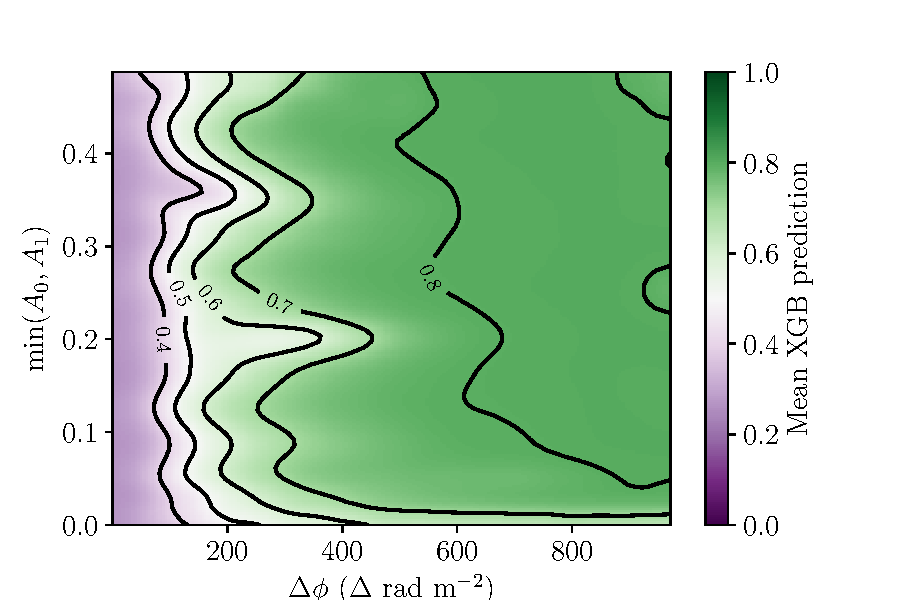
\includegraphics[width=\linewidth]{faraday-images/mean_xgb_prediction_dphi_amp.pdf}
        \caption{\label{fig:faraday-mean-xgb-pred}}
      \end{subfigure}
      \begin{subfigure}{\linewidth}
        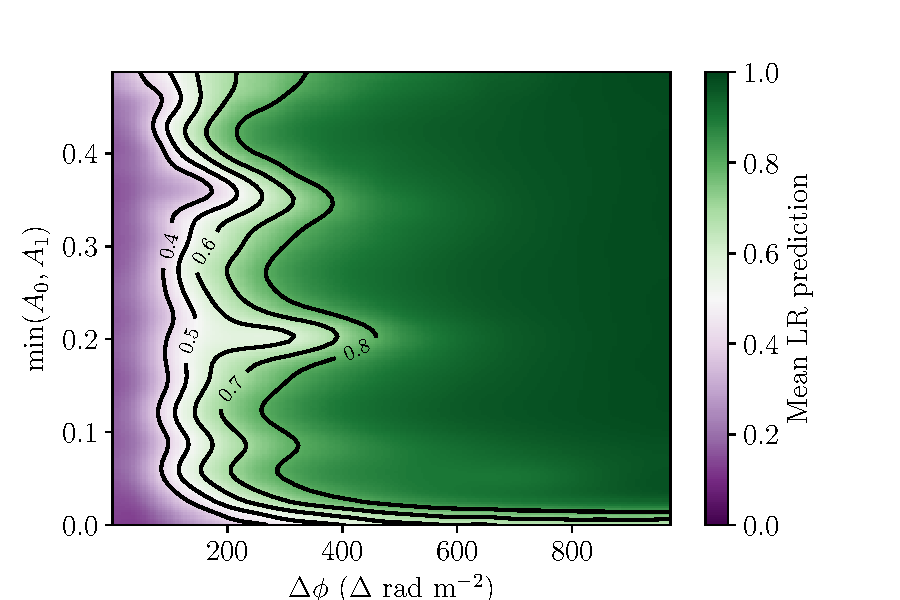
\includegraphics[width=\linewidth]{faraday-images/mean_lr_prediction_dphi_amp.pdf} 
        \caption{\label{fig:faraday-mean-lr-pred}}
      \end{subfigure}
      \caption{\label{fig:faraday-amps-dphi-mean} Mean prediction as a function of component depth separation and minimum component amplitude for (a) XGB and (b) LR.}
    \end{figure}

    As we know the true Faraday depths of the components in our simulation, we can investigate the behaviour of these classifiers as a function of physical properties. \autoref{fig:amps-dphi-mean} shows the mean classifier prediction as a function of component depth separation and minimum component amplitude. This is tightly related to the mean accuracy, as the entire plot domain contains complex spectra besides the left and bottom edge: by setting the threshold to a value on this plot, the accuracy will be one hundred per cent on the non-edge for all higher values. The most interesting feature of this plot is the curve, which arises from the RMSF.

    \begin{figure}
      \includegraphics[width=\linewidth]{faraday-images/acc_noise_xgb_lr.pdf}
      \caption{\label{fig:faraday-acc-noise} Mean accuracy as a function of noise level for both XGB and LR. Shading indicates the 95 per cent confidence level over 100 bootstrap samples. The dashed line marks the mean noise level in the simulation.}
    \end{figure}

    The accuracies of these classifiers are highly dependent on the noise level chosen for the simulation. We sampled noise level for each simulated FDF from a uniform distribution. Binning these simulated FDF based on their noise level lets us estimate the mean accuracy of our classifier as a function of noise level. The noise level is plotted against the mean accuracy in \autoref{fig:acc-noise}. While one may expect the accuracy to decrease with increasing noise, this isn't the case: the accuracy starts fairly high, peaks around $\sigma = 1.5$, and then decreases from this point. This is likely due to the classifier being trained on a range of noise levels. We have indicated the mean noise level in \autoref{fig:acc-noise}, which is near the peak accuracies for both classifiers.

    \begin{figure}
      \includegraphics[width=\linewidth]{faraday-images/acc_noise_xgb_lr_retrained.pdf}
      \caption{\label{fig:faraday-acc-noise-retrained} Mean accuracy after retraining as a function of noise level for both XGB and LR. Each classifier was retrained on each subset before prediction. Shading indicates the 95 per cent confidence level over 100 bootstrap samples.}
    \end{figure}

    To further investigate the effect of noise, we binned the simulated data by noise level and re-trained each classifier on the binned subsets. \autoref{fig:acc-noise-retrained} shows the mean accuracy as a function of noise. As expected, increasing noise is associated with decreasing accuracy when the classifier is not forced to generalise over a range of noises.

  \subsection{Results on observed FDFs}
  \label{sec:faraday-results-observed}

    \begin{figure}
      \centering
      \includegraphics[width=\linewidth]{faraday-images/pca.pdf}
      \caption{Principal component analysis for simulated data (coloured dots) with observations overlaid (white circles).}
      \label{fig:faraday-pca}
    \end{figure}

    We used our LR and XGB classifiers to estimate the probability that our 168 observed FDFs (\autoref{sec:observational-data}) were Faraday complex. As these classifiers were trained on simulated data, they face the issue of the `domain gap': the distribution of samples from a simulation differs from the distribution of real sources, and this affects performance on real data. Solving this issue is called `domain adaptation' and how to do this is an open research question in machine learning. Nevertheless, the features of our observations fall in the same region of feature space as the simulations (\autoref{fig:pca}) and so we expect reasonably good domain transfer.

    \begin{figure}
      \centering
      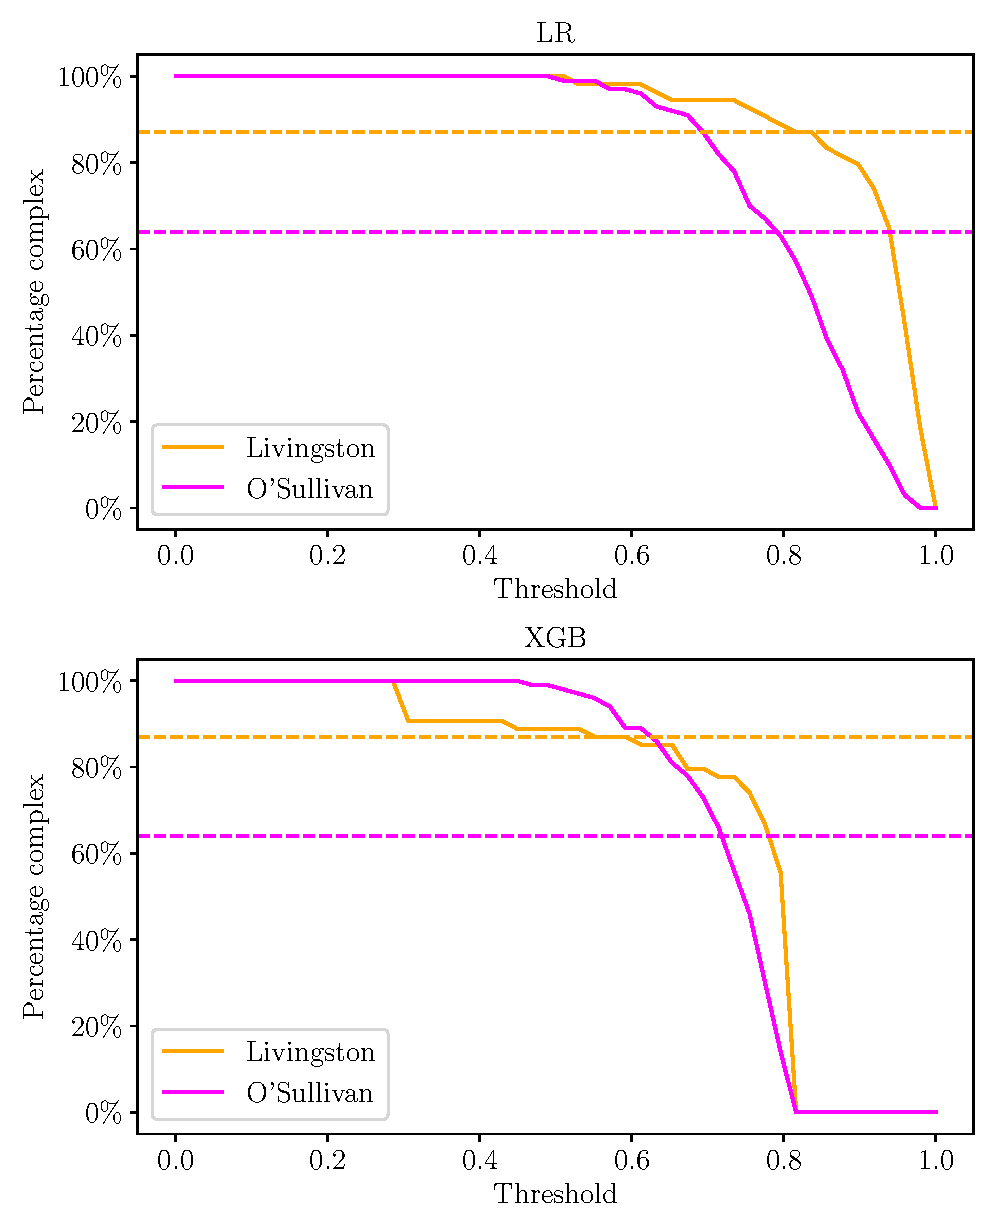
\includegraphics[width=\linewidth]{faraday-images/pc_complex_curves.pdf}
      \caption{Estimated rates of Faraday complexity for the Livingstone and O'Sullivan datasets as functions of threshold. The horizontal lines indicate the rates of Faraday complexity estimated by Livingston and O'Sullivan respectively.}
      \label{fig:faraday-complexity-rates}
    \end{figure}

    XGB predicted that 65 and 33 per cent of the Livingston and O'Sullivan sources were complex respectively. LR predicted that 60 and 31 per cent of the Livingston and O'Sullivan sources were complex respectively. This is in line with expectations that the Livingston data should have more Faraday complex sources than the O'Sullivan data due to their location near the galactic centre. However, Livingston et al. (in prep) found that 90 per cent of their sources were complex, and \citet{osullivan_broad-band_2017} found that 64 per cent of their sources were complex. This suggests that our classifiers are underestimating complexity, though it could also be the case that the methods used by Livingston and O'Sullivan overestimate complexity. Modifying the prediction threshold from 0.5 changes the estimated rate of Faraday complexity, and we show the estimated rates against threshold for both classifiers in \autoref{fig:complexity-rates}. Setting the threshold to 0.3 for LR and 0.4 for XGB would produce complexity rates much closer to those observed in both papers, but we chose to keep the threshold at 0.5 as this had the highest accuracy in the simulations.

    \begin{figure*}
      \centering
      \begin{subfigure}{0.45\linewidth}
        \includegraphics[width=\linewidth]{faraday-images/livingston_false_positive.pdf}
        \caption{Predicted complex.}
        \label{fig:faraday-livingston-false-positive}
      \end{subfigure}%
      \begin{subfigure}{0.45\linewidth}
        \includegraphics[width=\linewidth]{faraday-images/livingston_false_negative.pdf}
        \caption{Predicted simple.}
        \label{fig:faraday-livingston-false-negative}
      \end{subfigure}
      \begin{subfigure}{0.45\linewidth}
        \includegraphics[width=\linewidth]{faraday-images/osullivan_false_positive.pdf}
        \caption{Predicted complex.}
      \end{subfigure}%
      \begin{subfigure}{0.45\linewidth}
        \includegraphics[width=\linewidth]{faraday-images/osullivan_false_negative.pdf}
        \caption{Predicted simple.}
      \end{subfigure}
      \caption{Randomly-selected misclassified FDFs. (a) and (b) are from the Livingston dataset, and (c) and (d) are from the O'Sullivan dataset. (a) and (c) were misclassified as complex while (b) and (d) were misclassified as simple.}
      \label{fig:faraday-misclassified}
    \end{figure*}

    \autoref{fig:misclassified} shows four randomly-selected FDFs where the XGB prediction disagrees with the Livingston or O'Sullivan models. The complex FDFs in the Livingston dataset that were identified as simple by the classifier tend to have very different component amplitudes and a very high signal-to-noise main peak, while the simple FDFs identified as complex tend to be very noisy. \autoref{fig:all-observed-fdfs} shows every observed FDF ordered by estimated Faraday complexity alongside the models predicted by Livingston and O'Sullivan.

    \begin{figure*}
      \centering
      \includegraphics[width=\linewidth]{faraday-images/both_spectra.pdf}
      % \includegraphics[width=0.7\linewidth]{faraday-images/jack_spectra.pdf}
      \caption{The 168 observed FDFs ordered by XGB-estimated probability of being Faraday complex. Livingston-identified components are shown in orange while O'Sullivan-identified components are shown in magenta. Simpler FDFs are shown in purple while more complex FDFs are shown in green, and the numbers overlaid indicate the XGB estimate.},
      \label{fig:faraday-all-observed-fdfs}
    \end{figure*}

\section{Discussion}
\label{sec:faraday-discussion}

  Our results on observed FDFs show that our classifiers produce plausible results, with \autoref{fig:all-observed-fdfs} showing a clear trend of apparent complexity. In \autoref{sec:results-observed} we demonstrated that our classifiers predict lower rates of Faraday complexity than the methods of Faraday moments and QU-fitting employed by Livingston and O'Sullivan respectively. This makes sense in the context of our confusion matrices on the simulations (\autoref{tab:cm-lr} and \autoref{tab:cm-xgb}), which show that the main failure mode of the classifiers is misclassifying a complex source as simple, so we should expect a lower rate of complexity than the true complexity rate. This arises from the fact that some complex sources truly look simple, with very close Faraday components or very small amplitudes on the secondary component. \autoref{fig:livingston-false-negative} is an example of such a classification. Whether such sources should be considered complex is not clear, since for practical purposes they can be treated as simple: the RM estimated by assuming that the source is simple will be quite close to the RM at the location of the primary component, and thus would not negatively impact further data products such as an RM grid. Additionally, sources like these are almost certainly hidden in the presumably `simple' FDFs by the frequency range and spacing of the observations, just as how these complex sources would be hidden in lower-resolution observations. Issues like model overfitting (with QU-fitting) or high sensitivity to choice of noise cutoff (with RM-CLEAN and Faraday moments) may also inflate the rate of complexity in the O'Sullivan and Livingston models respectively, so we refrain from stating that either complexity estimation method is \emph{wrong}, just that they do not match. For any given source, both methods may produce plausible but disagreeing results.

  The domain gap is a problem that requires further research to solve. We have no good way to ensure that our simulation matches reality, so some amount of domain adaptation will always be necessary to train classifiers on simulated data and then apply these classifiers to real data. But with the low source counts in polarisation science (high-resolution spectropolarimetric data currently numbers in the few hundreds) any machine learning method will need to be trained on simulations. This is not just a problem in Faraday complexity estimation, and domain adaptation is also an issue faced in the wider astroinformatics community: large quantities of labelled data are hard to come by, and some sources are very rare \citep[e.g. gravitational wave detections or fast radio bursts;][]{zevin17gravityspy, gebhard19convolutional, agarwal20fetch}. Some aspects of the domain gap in our work are clear, such as our ignoring of internal and external Faraday dispersion. These aspects can be partly remedied in future work by including them in the simulations, though the distribution may still not match reality. However, our results are plausible and the distribution of our simulation well overlaps the distribution of our real data (\autoref{fig:pca}). Previous machine learning work \citep[e.g.][]{brown_classifying_2018} has not been run before on real FDF data, so this paper is the first example of the domain gap arising in Faraday complexity classification.

  The main way that our simulation accounts for non-modelled features of the observational data (e.g. a third component) is through noise. At its most extreme, a sufficiently noisy simple or complex FDF can match any observation. While this is not quite the case in our simulation, noise is the main mechanism that ensures the region of feature space that the simulation occupies covers that of the real data. This may result in unusual or unexpected results: for example, a 3-component source may be misidentified as a very noisy simple source. Improving the simulation (e.g. extension to more components) may reduce issues like these. However, this kind of misidentification is intrinsically a problem with complexity estimation anyway, as complex sources may conspire to appear as a wide range of viable models including simple \citep{sun15comparison}.

  Through this work we discovered that noise is a complicated and important issue in Faraday complexity estimation. One key question is how Faraday complexity estimators should behave as the noise increases: should high noise result in a complex prediction or a simple prediction, given that a complex or simple FDF would both be consistent with a noisy FDF? Occam's razor suggests that we should choose the simplest suitable model, and so increasing noise should lead to predictions of less complexity. This is not how our classifiers operate, however, as exemplified by \autoref{fig:livingston-false-positive}: high-noise FDFs are different to the model simple FDFs and so are predicted to be `not simple'. In some sense our classifiers are not looking for complex sources, but are rather looking for `not simple' sources. This is not the only issue related to noise in our work. \autoref{fig:acc-noise} demonstrates that the accuracy of our classifiers is dependent on the amount of noise in the simulated FDF in a surprising way: the correlation between noise and accuracy is not monotonic, and instead accuracy \emph{increases} as the noise increases up to the mean noise level of the training set. The classifier is forced to generalise over different amounts of noise with no good way to estimate how much noise is in a given FDF. This could be remedied by including noise as a feature, as suggested by \autoref{fig:acc-noise-retrained} which shows improved classifier behaviour when the training set was divided into different amounts of noise and the classifier was only trained and validated on FDFs with similar amounts of noise. But this is hard to generalise to real data: we would need not only a reliable noise estimate, but a reliable noise estimate that behaves in the same way to the simulated noise. We found that we needed very high noise ($\sigma \in [0, 3]$) to replicate the range of observed FDFs. The mean noise of the Livingston data was $0.028_{-0.022}^{+0.024}$, much lower than our simulated noise. This, combined with the fact that our simulated FDFs look very similar to the observed FDFs, suggests that either or both a) the injected noise and real noise have different units, or b) important aspects of the observed data are not captured by our simulation. This is another example of the domain gap in action and further research is required to unify the simulated and observed noise. The amount of noise can then be included as a feature for the classifier, which could greatly improve performance on both simulated and observed data.

  It is unclear what the effect of our simplifying assumptions (\autoref{sec:assumptions}) are on the effectiveness of our simulation. The three main simplifications we think may negatively affect our simulations are 1) limiting to two components, 2) assuming no external Faraday dispersion, and 3) assuming no internal Faraday dispersion (Faraday thickness). Future work will explore removing these simplifying assumptions, but will need to account for the increased difficulty in characterising the simulation with more components and no longer having Faraday screens as components. Additionally, more work will be required to make sure that the rates of internal and external Faraday dispersion match what might be expected from real sources, or risk making a simulation that has too large a range of consistent models for a given source: for example, a two-component source could also be explained as a sufficiently wide or resolved-out Faraday thick source or a three-component source with a small third component. This greatly complicates the classification task.

  Our classifiers are interpretable. The features are easy to understand and have clear relationship to the true simulation parameters (\autoref{fig:features-simparams}), and the classifiers themselves are simple enough that it is possible to understand how the classifier came to a given classification for a given source. LR is particularly simple, and similar enough in performance to XGB that it may be the preferable classifier for Faraday complexity estimation. We can examine its weights to find why it predicted a given FDF was simple or complex. For example, in \autoref{fig:misclassified}, a) was classified as complex due to its low maximum value of $|\hat F|$ and its high Euclidean distance from the simple manifold, b) and d) were both classified as simple due to their low Euclidean distance from the simple manifold, and c) was classified as complex due to its high maximum $|\hat F|$ and $W_2$ distance from the simple manifold (though the prediction is very close to the decision boundary because it has a low Euclidean distance from the simple manifold). Interpretability in a classifier is valuable in astronomy, as understanding the limitations and behaviour of our methods is important to ensure that any physical predictions we make from our results are sensible, well-motivated, and consistent with physics.

\section{Conclusion}
\label{sec:faraday-conclusion}

  We developed a simple, interpretable machine learning method for estimating Faraday complexity. Our interpretable features were derived by comparing observed FDFs to idealised simple FDFs, which we could determine both for simulated and real observations. We demonstrated the effectiveness of our method on both simulated and real data. Using simulated data, we found that our classifiers were 95 per cent accurate, with near perfect recall of Faraday simple sources (specificity). On simulated data with higher noise required to match our observations, we found that the accuracy dropped to 75 per cent, though the amount of noise can be reduced in future by further development of the simulation. Evaluating our classifiers on real data gave plausible results. Future work will need to narrow the domain gap to improve transfer of classifiers trained on simulations to real, observed data.

  % If we were to run our classifiers at scale on the upcoming POSSUM survey, how would the limitations presented in \autoref{sec:results-simulated} affect derived statistics of Faraday complexity? 

  % \begin{itemize}
  %   \item Mention Brown cuts. What are the implications for POSSUM if we were to use our classifier? How does this affect what we can detect and can't?
  % \end{itemize}

  % \begin{itemize}
  %   \item (10) is a good example of noise being important but we can't explicitly factor it in yet - this is two peaks that are very different scales
  %   \item (27) is funky, we get a smooth-looking FDF but it's not obviously two peaks. see also (47)
  %   \item (38) has $\phi_s$ outside of the range! but it still looks good
  % \end{itemize}